\documentclass{article}

\usepackage{amsmath}
\usepackage{graphicx}
\usepackage{subcaption}
\usepackage{setspace}
\usepackage[backend=bibtex,style=verbose-trad2]{biblatex}
\usepackage{siunitx}
\usepackage{multirow}
\usepackage{booktabs}
\usepackage{longtable}
\usepackage{listings}
\usepackage{color}
\usepackage{hyperref}
\usepackage{enumitem}

\title{My first document}
\date{2018-09-29}
\author{Marek Dudek}

\setcounter{tocdepth}{1}

\bibliography{dummy}

\sisetup{
    round-mode = places,
    round-precision = 2
}

\renewcommand\lstlistingname{Quelltext}

\lstset{
    language=Perl,
    basicstyle=\small\sffamily,
    numbers=left,
    numberstyle=\tiny,
    frame=tb,
    tabsize=4,
    columns=fixed,
    showstringspaces=false,
    showtabs=false,
    keepspaces,
    commentstyle=\color{red},
    keywordstyle=\color{blue}
}

\begin{document}

    \pagenumbering{gobble}
    \maketitle

    \newpage
    \doublespacing
    \tableofcontents
    \singlespacing

    \newpage
    \pagenumbering{arabic}

    \section{Section}
    Hello World!
    \subsection{Subsection}
    Structuring a document is easy!
    \subsubsection{Subsubsection}
    This is sub-subsection.
    \paragraph{Paragraph}
    This is a paragraph.
    \subparagraph{Subparagraph}
    This is a subparagraph.

    \section{Another section}

    \section{Math}

	    \begin{equation}
		f(x) = x^2
	    \end{equation}
	    \begin{equation*}
		f(x) = x^2
	    \end{equation*}

        This formula $f(x) = x^2$ is an example of embedded formula.

    \begin{align*}
 	1 + 2 &= 3\\
 	1 &= 3 - 2
    \end{align*}

    \begin{align*}
 	f(x) &= x^2\\
	g(x) &= \frac{1}{x}\\
	F(x) &= \int^a_b \frac{1}{3}x^3\\
	G(x) &= \frac{1}{\sqrt{x}}
    \end{align*}

    \begin{equation*}
	    \begin{matrix}
		1 & 0\\
		0 & 1
	    \end{matrix}
    \end{equation*}

    \begin{equation*}
	    \begin{bmatrix}
		1 & 0\\
		0 & 1
	    \end{bmatrix}
    \end{equation*}

    \begin{equation*}
	[
	\begin{matrix}
	    1 & 0\\
	    0 & 1
	\end{matrix}
	]
    \end{equation*}

    \begin{equation*}
	\left[
	\begin{matrix}
	    1 & 0\\
	    0 & 1
	\end{matrix}
	\right]
    \end{equation*}

    \begin{equation*}
	\left(\frac{1}{\sqrt{x}}\right)
    \end{equation*}

    This is $\lambda$!

    \newpage

    \section{Pictures}

    \begin{figure}[h!]
	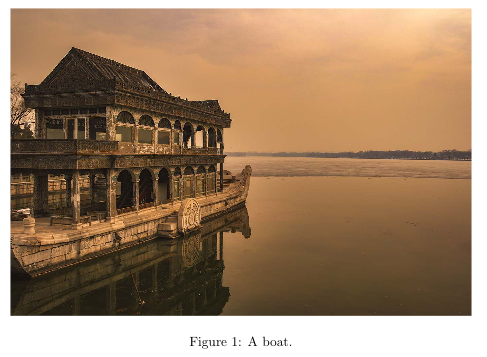
\includegraphics[width=\linewidth]{images/boat.png}
	\caption{A boat.}
	\label{fig:boat1}
    \end{figure}

    Figure \ref{fig:boat1} shows a boat.

    \begin{figure}[h!]
	\centering
	\begin{subfigure}[b]{0.4\linewidth}
		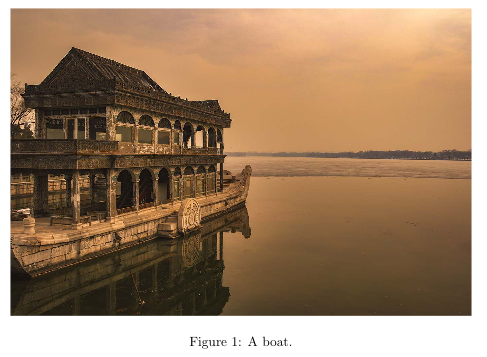
\includegraphics[width=\linewidth]{images/boat.png}
		\caption{A boat.}
	\end{subfigure}
	\begin{subfigure}[b]{0.4\linewidth}
		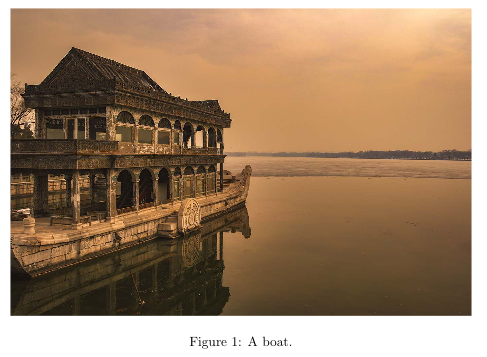
\includegraphics[width=\linewidth]{images/boat.png}
		\caption{Another boat.}
	\end{subfigure}
	\caption{The same boat two times.}
	\label{fig:twoboats}
    \end{figure}

    \newpage

    \section{Tables}

    \begin{table}[h!]
	\caption{Dummy table}
    \end{table}

    \newpage

    \section{Using BibTeX}

    Random citation \autocite[1]{DUMMY:1} embedded in text.

    \newpage

    \section{Footnotes}

    \paragraph{}
    This is some example text\footnote{\label{myfootnote}Hello footnote!} with footnote.

    \paragraph{}
    Some other text.

    \paragraph{}
    I'm refering to footnote \ref{myfootnote}.

    \newpage

    \section{Tables}

    \begin{table}[h!]
	\begin{center}
	    \caption{Your first table.}
	    \label{tab:table1}
	    \begin{tabular}{l|S|r|l}
		\textbf{Value 1} & \textbf{Value 2} & \textbf{Value 3} & \textbf{Value 4} \\
		\hline
		$\alpha$         & $\beta$          & $\gamma$         & $\delta$         \\
		\hline
		1 & 1110.1    & a & e \\
		2 & 10.1      & b & f \\
		3 & 23.113231 & c & g \\
		4 & 25.113231 & d & h \\
		\hline
	    \end{tabular}
	\end{center}
    \end{table}    

    \paragraph{}
    Another table

    \begin{table}[h!]
	\begin{center}
	    \caption{Multicolumn table.}
	    \label{tab:table2}
	    \begin{tabular}{l|S|r}
		\toprule
		Column 1 & Column 2 & Column 3 \\
		\midrule
		$\alpha$ & $\beta$  & $\gamma$ \\
		\midrule
		\multicolumn{2}{c|}{12} & a \\
		\midrule
		2 & 10.1 & b \\ 
		\midrule
		3 & \multicolumn{2}{c}{\multirow{2}{*}{1234}} \\ 
		4 & \multicolumn{2}{c}{} \\ 
		\midrule
		5 & 40.4 & e \\ 
		\bottomrule
	    \end{tabular}
	\end{center}
    \end{table}

    \paragraph{}

    Long table

    \begin{longtable}[c]{l|S|r}
	\caption{Long table.}
	\label{tab:table3}\\
	\toprule
	Column 1 & \textbf{Column 2} & Column 3 \\
	$\alpha$ & $\beta$  & $\gamma$ \\
	\midrule
	\endfirsthead
	\toprule
	Column 1 & \textbf{Column 2} & Column 3 \\
	\midrule
	\endhead
	2 & 10.1 & b \\ 
	2 & 10.1 & b \\ 
	2 & 10.1 & b \\ 
	2 & 10.1 & b \\ 
	2 & 10.1 & b \\ 
	2 & 10.1 & b \\ 
	2 & 10.1 & b \\ 
	2 & 10.1 & b \\ 
	2 & 10.1 & b \\ 
	5 & 40.4 & e \\ 
	2 & 10.1 & b \\ 
	5 & 40.4 & e \\ 
	5 & 40.4 & e \\ 
	2 & 10.1 & b \\ 
	5 & 40.4 & e \\ 
	2 & 10.1 & b \\ 
	5 & 40.4 & e \\ 
	2 & 10.1 & b \\ 
	5 & 40.4 & e \\ 
	5 & 40.4 & e \\ 
	2 & 10.1 & b \\ 
	2 & 10.1 & b \\ 
	2 & 10.1 & b \\ 
	2 & 10.1 & b \\ 
	5 & 40.4 & e \\ 
	2 & 10.1 & b \\ 
	5 & 40.4 & e \\ 
	5 & 40.4 & e \\ 
	2 & 10.1 & b \\ 
	5 & 40.4 & e \\ 
	2 & 10.1 & b \\ 
	5 & 40.4 & e \\ 
	2 & 10.1 & b \\ 
	5 & 40.4 & e \\ 
	5 & 40.4 & e \\ 
	2 & 10.1 & b \\ 
	2 & 10.1 & b \\ 
	2 & 10.1 & b \\ 
	2 & 10.1 & b \\ 
	5 & 40.4 & e \\ 
	2 & 10.1 & b \\ 
	5 & 40.4 & e \\ 
	5 & 40.4 & e \\ 
	2 & 10.1 & b \\ 
	5 & 40.4 & e \\ 
	2 & 10.1 & b \\ 
	5 & 40.4 & e \\ 
	2 & 10.1 & b \\ 
	5 & 40.4 & e \\ 
	5 & 40.4 & e \\ 
	2 & 10.1 & b \\ 
	2 & 10.1 & b \\ 
	2 & 10.1 & b \\ 
	2 & 10.1 & b \\ 
	5 & 40.4 & e \\ 
	2 & 10.1 & b \\ 
	5 & 40.4 & e \\ 
	5 & 40.4 & e \\ 
	2 & 10.1 & b \\ 
	5 & 40.4 & e \\ 
	2 & 10.1 & b \\ 
	5 & 40.4 & e \\ 
	2 & 10.1 & b \\ 
	5 & 40.4 & e \\ 
	5 & 40.4 & e \\ 
	2 & 10.1 & b \\ 
	2 & 10.1 & b \\ 
	2 & 10.1 & b \\ 
	2 & 10.1 & b \\ 
	5 & 40.4 & e \\ 
	2 & 10.1 & b \\ 
	5 & 40.4 & e \\ 
	5 & 40.4 & e \\ 
	2 & 10.1 & b \\ 
	5 & 40.4 & e \\ 
	2 & 10.1 & b \\ 
	5 & 40.4 & e \\ 
	2 & 10.1 & b \\ 
	5 & 40.4 & e \\ 
	5 & 40.4 & e \\ 
	2 & 10.1 & b \\ 
	2 & 10.1 & b \\ 
	2 & 10.1 & b \\ 
	2 & 10.1 & b \\ 
	5 & 40.4 & e \\ 
	2 & 10.1 & b \\ 
	5 & 40.4 & e \\ 
	5 & 40.4 & e \\ 
	2 & 10.1 & b \\ 
	5 & 40.4 & e \\ 
	2 & 10.1 & b \\ 
	5 & 40.4 & e \\ 
	2 & 10.1 & b \\ 
	5 & 40.4 & e \\ 
	5 & 40.4 & e \\ 
	2 & 10.1 & b \\ 
	5 & 40.4 & e \\ 
	2 & 10.1 & b \\ 
	2 & 10.1 & b \\ 
	5 & 40.4 & e \\ 
	2 & 10.1 & b \\ 
	5 & 40.4 & e \\ 
	5 & 40.4 & e \\ 
	2 & 10.1 & b \\ 
	5 & 40.4 & e \\ 
	2 & 10.1 & b \\ 
	5 & 40.4 & e \\ 
	2 & 10.1 & b \\ 
	5 & 40.4 & e \\ 
	5 & 40.4 & e \\ 
	2 & 10.1 & b \\ 
	5 & 40.4 & e \\ 
	\bottomrule
    \end{longtable}

    \newpage

    \section{Code listing}
    \subsection{Embedded}

    \begin{lstlisting}
#!/usr/bin/perl
print S(@ARGV);sub S{$r=(@_[0]%4==0&&@_[0]%100!=0)||@_[0]%400=0;}
    \end{lstlisting}

    \subsection{Imported from file}

    \lstinputlisting{script.pl}

    \newpage

    \section{Hyperlinks}

    This is my link: \href{http://www.onet.pl}{Onet}.

    \newpage

    \section{Lists}
    
    \subsection{Unordered list}

    \begin{itemize}
        \item default
        \item[--] dash
        \item[$-$] dash
        \item[$\ast$] asterix 
        \item[$\lambda$] any math character
    \end{itemize}

    \subsection{Ordered list}

    \begin{enumerate}
        \item One
        \item Two
        \item Three
    \end{enumerate}

    \subsection{Ordered list, roman style}

    \begin{enumerate}[label=(\roman*)]
        \item One
        \item Two
        \item Three
    \end{enumerate}

    \subsection{Ordered list, arabic style}

    \begin{enumerate}[label=(\arabic*)]
        \item One
        \item Two
        \item Three
    \end{enumerate}

    \subsection{Ordered list, alphabetical style}

    \begin{enumerate}[label=(\alph*)]
        \item One
        \item Two
        \item Three
    \end{enumerate}


    \subsection{Nested list}

    \begin{enumerate}
        \item One
            \begin{enumerate}
                \item Two
                \item Three
                \item Four
            \end{enumerate}
        \item Five
        \item Six
    \end{enumerate}

    \newpage
    
    \begin{appendix}
	\listoffigures
	\listoftables
    \end{appendix}

\end{document}
